\documentclass{beamer}
\usepackage{fontawesome5} % Add fancy icons
\usepackage{tikz}
\usetikzlibrary{positioning}
\usepackage{xcolor}
\usepackage{graphicx}
\usepackage{biblatex}
\addbibresource{citation.bib}
\AtBeginBibliography{\small}

\usetheme[progressbar=frametitle]{metropolis}
\setbeamertemplate{frame numbering}[fraction]
%\setbeamertemplate{frametitle}{\strut\insertframetitle\strut\hfill\includegraphics[width=1cm]{logo}}
%\setbeamertemplate{frame footer}{Robet Koch Institute \hspace{30pt} CQ Beratung\&Bilding}
%\setbeamertemplate{frame footer}{\includegraphics[width=.5cm]{logo}}
\setbeamertemplate{frame footer}{\insertshortauthor \hspace{60pt}\insertshortinstitute \hspace{50pt} \insertdate}
\setbeamerfont{page number in head/foot}{size=\tiny}
\setbeamercolor{footline}{fg=gray}
%\setbeamercolor{footline}{bg=gray}
\setbeamercolor{background canvas}{bg=white}
\useoutertheme{metropolis}

\useinnertheme{metropolis}
\usefonttheme{metropolis}
%\usecolortheme{monarca}
\usecolortheme{spruce}
\definecolor{mygreen}{rgb}{.125,.5,.25}
%\definecolor{awesome}{rgb}{1.0, 0.13, 0.32}
\usecolortheme[named=mygreen]{structure}
%\usecolortheme[named=awesome]{structure}

\definecolor{myyellow}{rgb}{1.0, 0.83, 0.0}
\definecolor{uclagold}{rgb}{1.0, 0.7, 0.0}
%\usecolortheme[named=uclagold]{structure}

\title[Short Title]{Internship}
\subtitle{Automated HIV-1 Genotyping}
\author{\vspace{50pt} Vera Rykalina}
\institute{CQ Beratung\&Bildung/Robert Koch Institute}
\date{\today}


%\definecolor{myblue}{RGB}{29,57,127}
%\newcommand{\seticon}[1]{\textcolor{mygreen}{\csname #1\endcsname}}

\definecolor{citrine}{rgb}{0.89, 0.82, 0.04}
\definecolor{timberwolf}{rgb}{0.86, 0.84, 0.82}
\definecolor{whitesmoke}{rgb}{0.96, 0.96, 0.96}

\begin{document}
\metroset{block=fill}
%\setbeamercolor{block title}{bg=timberwolf, fg=black}
%\setbeamercolor{block body}{fg=black,bg=whitesmoke}



\begin{frame}[noframenumbering,plain, standout]
\titlepage
\end{frame}

\section{Outline}
\begin{frame}{Outline}
%\begin{tikzpicture}[overlay, remember picture]
%\node[above left=8.4cm and 0.2cm of current page.south east] %{\includegraphics[width=1cm]{logo}};
%\end{tikzpicture}
\tableofcontents
\end{frame}



\section{Introduction}
\begin{frame}{INTRO: HIV-1 \cite{toxins14020138}} 
\begin{figure}
\centering
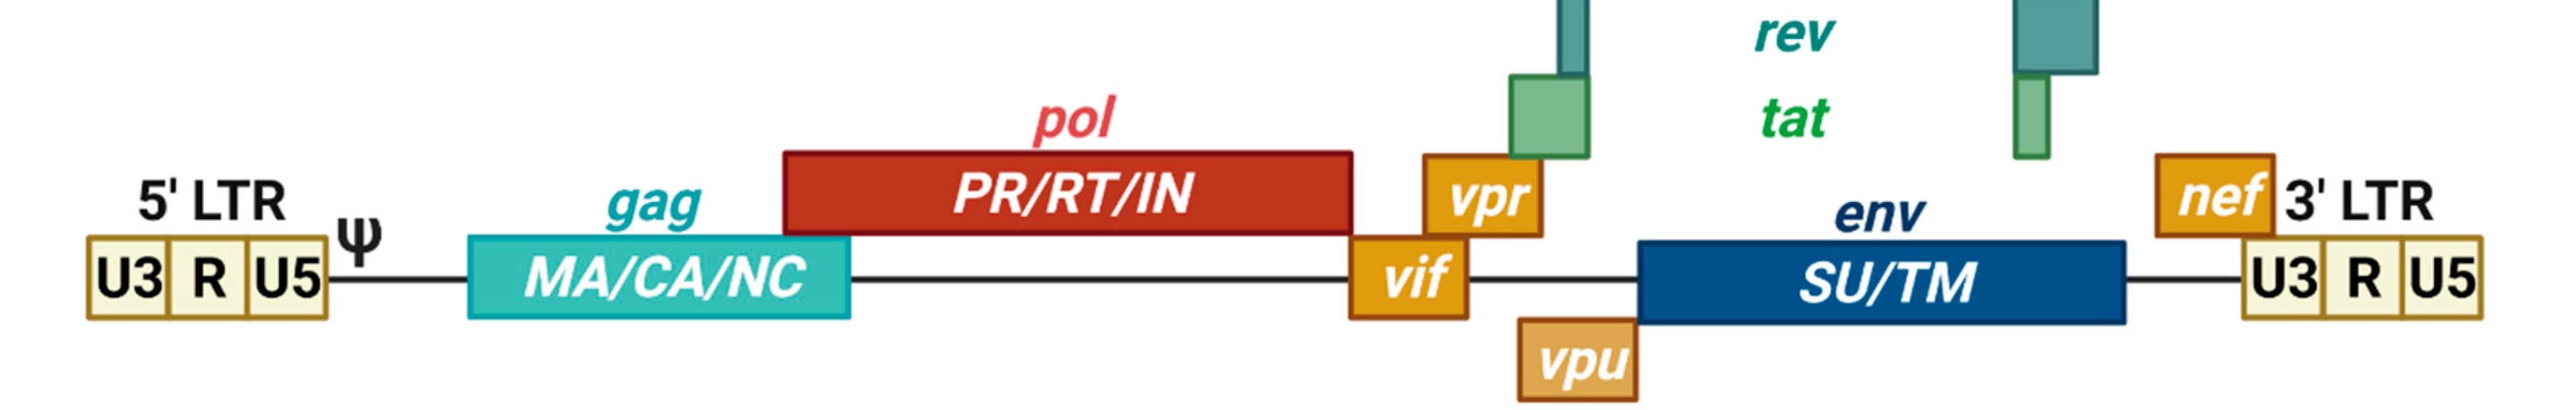
\includegraphics[scale=0.07]{toxins-14-00138-g001.png}\\
- - - - - - - - - - - - - - - - - - - - - - - - - - - - - - - - - - - - -\\
\vspace{6pt}
\centering
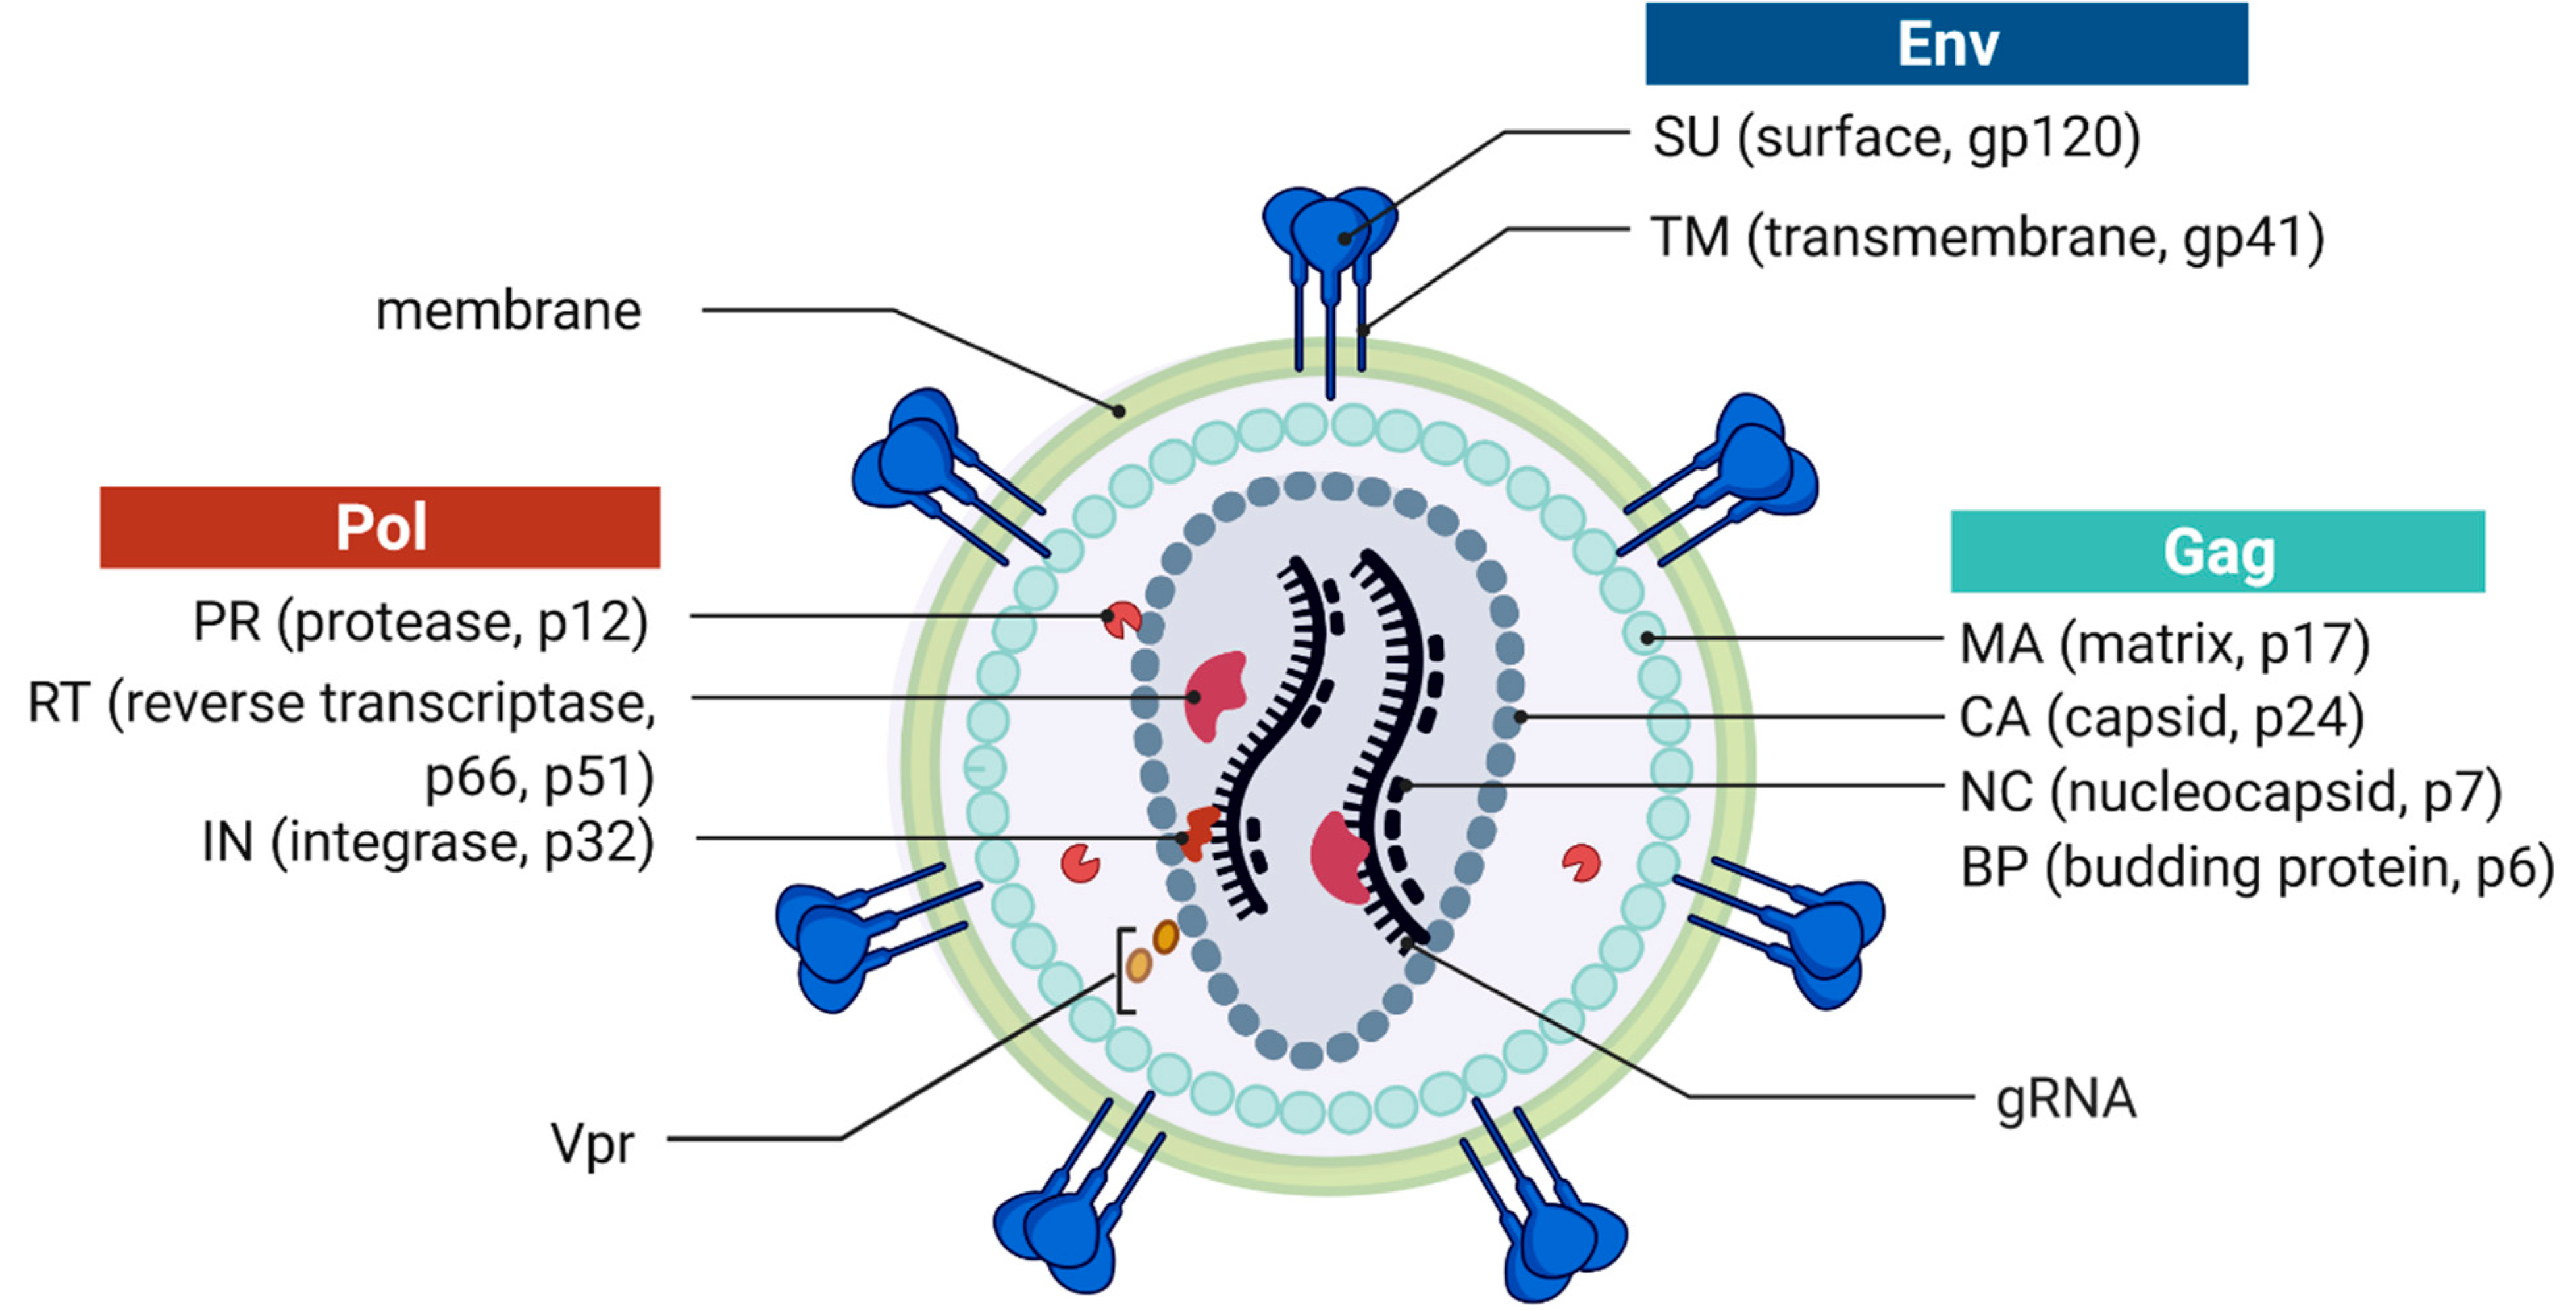
\includegraphics[scale=0.07]{toxins-14-00138-g002.png}
\end{figure}
\end{frame}




\begin{frame}{Introduction}
Subtyping is performed by using a combination of the following tools.\\
\vspace{10pt}
\begin{block}{\textbf{Online Subtyping Tools}}
\begin{itemize}
\item STANFORD (sierrapy)\\ 
\href{https://hivdb.stanford.edu/hivdb/by-sequences/}{https://hivdb.stanford.edu/hivdb/by-sequences/}
\item COMET (https requests)\\
\href{https://comet.lih.lu/}{https://comet.lih.lu/}
\item REGA (manual)\\ 
\href{https://www.genomedetective.com/app/typingtool/hiv}{https://www.genomedetective.com/app/typingtool/hiv}
\end{itemize}
\end{block}  
\end{frame}


\begin{frame}{Introduction}
\begin{block}{\textbf{HIV-1 Groups}}
Human immunodeficiency virus (HIV) displays an extraordinary genetic diversity with four distinct groups: 
\begin{itemize}
\item M (major)
\item O (outlier)
\item N (non M/O)
\item P (putative)
\end{itemize}
\end{block}  
\end{frame}



\begin{frame}{Introduction}
\textcolor{magenta}{HIV-1 Subtypes}\\
Within the major M Group are 9 different subtypes, at least 98 circulating recombinant forms (CRFs), and multiple unique recombinant forms (URF).
\begin{columns}[onlytextwidth]
\column{0.5\textwidth}

\begin{itemize}
\item {A (A1, A2, A3, A4, A5, A6)}
\item {B}
\item {C}
\item {D}
\item {F (F1, F2)}
\end{itemize}
\hspace{50pt}
\column{0.4\textwidth}

\begin{itemize}
\item {G}
\item {H}
\item {J}
\item {K}
\end{itemize}

\end{columns}
\vspace{5pt}
\centering
\footnotesize \href{http://www.hiv.lanl.gov/content/sequence/HIV/CRFs/CRFs.html}{http://www.hiv.lanl.gov/content/sequence/HIV/CRFs/CRFs.html}
\centering
\end{frame}


\section{Analysis}
\begin{frame}{Analysis}
\centering
\textcolor{magenta}{SUBTYPING (Toolwise)}
\vspace{10pt}
\centering
\begin{columns}[onlytextwidth]
\column{0.4\textwidth}
\begin{tabular}{|c|c|}
\hline 
ID & PR, RT \\ 
\hline 
1 & A \\ 
\hline 
2  & B \\ 
\hline 
... & ... \\ 
\hline 
n & F \\ 
\hline 
\end{tabular}
\column{0.30\textwidth}
\begin{tabular}{|c|c|}
\hline 
ID & IN \\ 
\hline 
1 & A \\ 
\hline 
2  & B \\ 
\hline 
... & ... \\ 
\hline 
n & F \\ 
\hline 
\end{tabular}
\column{0.3\textwidth}
\begin{tabular}{|c|c|}
\hline 
ID & ENV \\ 
\hline 
1 & A \\ 
\hline 
2  & B \\ 
\hline 
... & ... \\ 
\hline 
n & F \\ 
\hline 
\end{tabular}
\end{columns}
\end{frame}


\begin{frame}{Analysis}
\centering
\textcolor{magenta}{SUBTYPING (Fragmentwise)}\\
\vspace{10pt}
\begin{tabular}{|c|c|c|c|}
 \hline 
 ID & REGA & STANFORD & COMET \\ 
 \hline 
 1 & B & B & B \\ 
 \hline 
 2 & G & CRF02\_AG & G (check for 02\_AG) \\ 
 \hline 
 ... & ... & ... & ... \\ 
 \hline 
 n & CRF11\_cpx & A + J  & CRF11\_cpx \\ 
 \hline 
 \end{tabular} 
\end{frame}




\begin{frame}[t]{Customer's prefereces} \vspace{5pt}
\centering
\begin{figure}
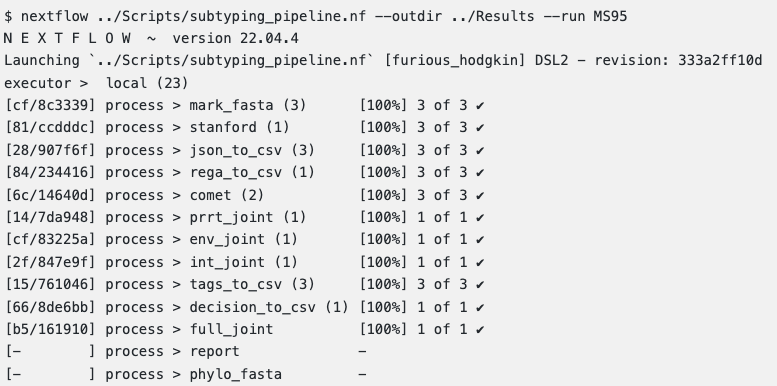
\includegraphics[scale=0.4]{nf.png}
\centering
\end{figure}
\end{frame}



\begin{frame}[t]{Predicting sales volume} \vspace{30pt}
\begin{columns}[onlytextwidth]
\column{0.5\textwidth}
\centering
\begin{figure}
%\includegraphics[scale=0.3]{s1}
%\caption{Brand preference}
\centering
\end{figure}
\column{0.5\textwidth}
\centering
\begin{figure}
%\includegraphics[scale=0.3]{s2}
%\caption{Least frequent items}
\centering
\end{figure}
\end{columns}
\vspace{10pt}
\centering
\begin{itemize}
\item Inability to specify product but product type.
\end{itemize}
\centering
\end{frame}


\begin{frame}[t]{Impact of Service and Customer Reviews} \vspace{4pt}
\centering
\begin{figure}
%\includegraphics[scale=0.4]{impactR}
%\caption{Rank of top 10 frequent items (absolute)}
\centering
\end{figure}
\vspace{10pt}
\centering
\begin{itemize}
\item Number of reviews is of great benefit to sales volume
\end{itemize}
\centering
\end{frame}


\begin{frame}[t]{TOOLS} \vspace{20pt}
\begin{columns}[onlytextwidth]
\column{0.5\textwidth}
\begin{flushleft}
\begin{figure}

\includegraphics[scale=0.25]{bash_logo.png}
\end{figure}
%\vspace{10pt}
\begin{figure}

\includegraphics[scale=0.2]{nextflow_logo.png}
\end{figure}
\begin{figure}

\includegraphics[scale=0.2]{python_logo.png}
\end{figure}
\begin{figure}

\includegraphics[scale=0.1]{git_logo.png}
\end{figure}
%\vspace{5pt}
\end{flushleft}
\column{0.5\textwidth}
\centering
\begin{itemize}
\vspace{5pt}
\item \footnotesize sierrapy, miller, mafft, iqtree
\vspace{20pt}
\item \footnotesize DSL2
\vspace{20pt}
\item  \footnotesize sys, re, collections, requests\\ pandas, time, wrap, json, bio
\vspace{20pt}
\item \footnotesize GitHub

\end{itemize}
\centering
\end{columns}
%The final value used for the model was k = 33.
\end{frame}


\begin{frame}[t]{REPO} \vspace{20pt}
\centering
\begin{figure}

\includegraphics[scale=0.2]{octocat.png}\\
\vspace{10pt}
\footnotesize \faIcon{github} \href{https://github.com/vera-rykalina/rki}{https://github.com/vera-rykalina/rki}
\centering
\end{figure}
\end{frame}

\begin{frame}{Transactional Data}
\begin{flushleft}
\textbf \footnotesize Acquisition
\end{flushleft}
\begin{itemize}
\item \footnotesize Complementary profile of both companies (Electronidex is more focused on high end products and Blackwell on lower end).
\item \footnotesize Blackwell could expand its customer database (9800 new clients)
\item \footnotesize Low frequent products of Electronidex could be easily sold by Blackwell
\item \footnotesize Due to financial difficulties Electronidex is a bargain
\item \footnotesize Inability to directly collate Electronidex's and Blackwell's (5 product match only)
\end{itemize}

\begin{columns}[onlytextwidth]
\column{0.5\textwidth}
\centering
\begin{figure}
%
\includegraphics[scale=0.2]{nextflow_logo.png}
\end{figure}
\centering
\vspace{0.5pt}
\column{0.5\textwidth}
\centering
\begin{figure}
%\includegraphics[scale=0.23]{LFI}
\centering
\end{figure}
\end{columns}

\end{frame} 


\begin{frame}[t]{Carbon} 
\vspace{4pt}
\begin{figure}
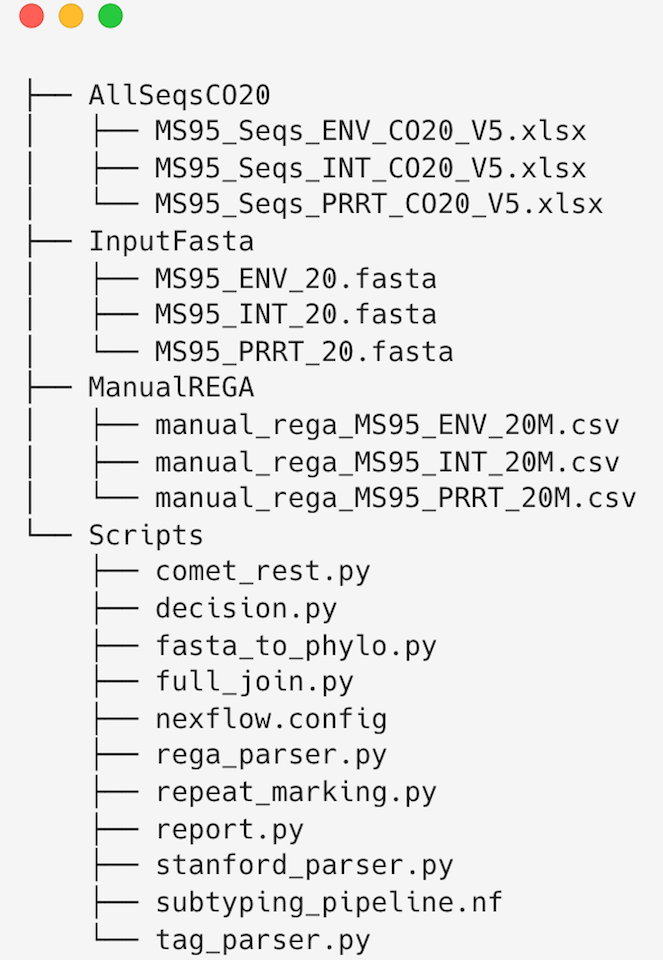
\includegraphics[scale=0.2]{tree.png}
\end{figure}
\end{frame}


\begin{frame}[t]{IQTREE} 
\vspace{4pt}
\begin{figure}
\includegraphics[scale=0.7]{MS95_PRRT_20M_highlighted.treefile.pdf}
\end{figure}
\end{frame}


\section{Conclusions}
\begin{frame}[t]{Conclusions} 
\begin{itemize}
\item Need to increase amount of data
\item Data quality investment (Demographic \& Historical)
\item New marketing stratigies based on clients preferences
\item Campaigns to induce customers to write reviews
\item Development of Recommender System
\item More transaction data to make a decision concerning acquisition
\end{itemize}
\begin{tikzpicture}[overlay, remember picture]
%\node[above left=1.5cm and 2.5cm of current page.south east] {\includegraphics[width=1.5cm]{logo}};
\end{tikzpicture}
\end{frame}


\begin{frame}[noframenumbering, plain, standout]
\huge Thank you!

\begin{center}
\begin{tabular}{c@{~}l@{~}l}
\small \faIcon{mobile-alt}& \small Phone: & \small +49 176 412 55 071\\
\small \faIcon[regular]{envelope}          & \small Email:    & \small \href{verarykalina@gmail.com}{verarykalina@gmail.com} \\
\small \faIcon{linkedin} & \small LinkedIn: & \small \href{https://www.linkedin.com/in/vera-rykalina-6b005728}{https://www.linkedin.com/in/vera-rykalina-6b005728}\\
\end{tabular}
\end{center}
\end{frame}



\begin{frame}[noframenumbering, plain, standout]
\huge Questions?
\end{frame}


% Add bibliography frame
\begin{frame}[allowframebreaks,plain,noframenumbering]
\printbibliography
\end{frame}

\end{document}
